\documentclass{beamer}
\usepackage{../../typesetting/styles/slide-zh}

% Document information
\title{\LARGE{周报}}
\subtitle{}
\author{}
\date{2025-04-14}

\begin{document}

% Title frame
\begin{frame}
  \titlepage
\end{frame}

% Outline frame
\begin{frame}{大纲}
  \tableofcontents
\end{frame}

\section{论文写作}
\begin{frame}{架构图优化}
  \begin{block}{优化内容}
    \begin{itemize}
      \item 新版SLH-DSA签名流程图结构更简洁明了
      \item 改进视觉层次与元素关系表达
      \item 更清晰展示ATA与FLP之间关系
    \end{itemize}
  \end{block}
  \begin{columns}[c]
    \column{0.48\textwidth}
    \centering
    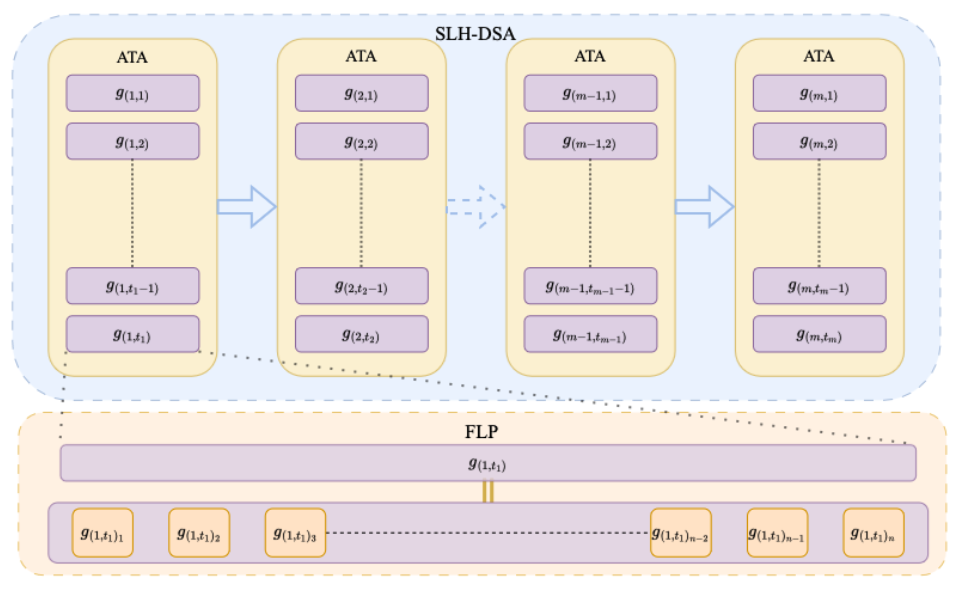
\includegraphics[width=\linewidth]{fig/arch_old.png}\\
    \footnotesize{左:原始流程图}
    \column{0.04\textwidth}
    % 空列用于间隔
    \column{0.48\textwidth}
    \centering
    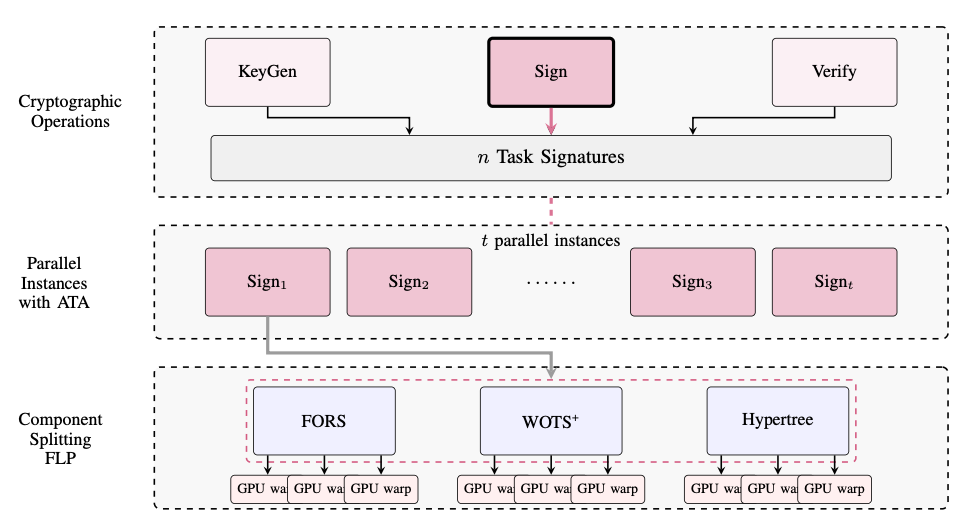
\includegraphics[width=\linewidth]{fig/arch.png}\\
    \footnotesize{右:改进后流程图}
  \end{columns}
\end{frame}

\section{FLP写作与实验}
\begin{frame}{FLP部分撰写与实验}
  \begin{block}{函数级并行(FLP)}
    \begin{itemize}
      \item FLP为Thread-Adaptive架构的重要组成部分
      \item 主要策略:
        \begin{itemize}
          \item WOTS$^+$并行化:$l$个哈希链并发计算
          \item FORS并行化:$k \times 2^a$密钥元素并行生成
          \item Hypertree并行化:跨$d$层多Merkle树并发构建
        \end{itemize}
      \item 合理利用合并内存访问与共享内存
    \end{itemize}
  \end{block}
\end{frame}

\begin{frame}{FLP实验结果}
  \begin{block}{签名操作延迟分布(SPHINCS$^+$-128f)}
    \begin{center}
      \scriptsize
      \begin{tabular}{lcc}
        \toprule
        \textbf{组件} & \textbf{延迟 (ms)} & \textbf{占总时间百分比} \\
        \midrule
        WOTS$^+$ Sign & 1.857 & 0.35\% \\
        FORS Sign & 29.371 & 5.58\% \\
        Hypertree Sign & \textcolor{red}{495.252} & \textcolor{red}{94.07\%} \\
        \midrule
        总签名延迟 & 526.48 & 100.00\% \\
        \bottomrule
      \end{tabular}
    \end{center}
  \end{block}
  \begin{itemize}
    \item Hypertree构建占据签名延迟主导地位(94.07\%)
  \end{itemize}
\end{frame}

\begin{frame}{老师评语}
  \begin{alertblock}{图2过大,一定要小而紧凑,多学学trans期刊绘图}
    继续对图表进行优化
  \end{alertblock}

  \vfill

  \begin{block}{下周工作计划}
    \begin{itemize}
      \item 全面检查论文符号一致性与潜在错误
      \item 进一步优化关键图表和实验结果呈现方式
    \end{itemize}
  \end{block}
\end{frame}

% References
% \begin{frame}
%   \frametitle{参考文献}
%   \bibliographystyle{alpha}
%   \bibliography{../../paper}
% \end{frame}

\end{document}
